\documentclass{article}

% content/resources/templates/preamble.tex
\usepackage[margin=0.6in]{geometry}
\author{Milav Dabgar}
\usepackage{amsmath,amssymb,amsthm}
\usepackage{booktabs}
\usepackage{multirow}
\usepackage{xcolor}
\usepackage{tcolorbox}
\tcbuselibrary{breakable,skins}
\usepackage[colorlinks=true,linkcolor=blue]{hyperref}
\usepackage{titlesec}
\usepackage{enumitem}
\usepackage{tikz}
\usepackage{pgfplots}
\usepackage{circuitikz}
\usepackage[version=4]{mhchem}
\usepackage{longtable}
\usepackage{array}
\usepackage{float}
\usepackage{caption}
\usepackage{listings}

\lstset{
  basicstyle=\small\ttfamily,
  breaklines=true,
  breakatwhitespace=false,
  postbreak=\mbox{\textcolor{red}{$\hookrightarrow$}\space},
  float=false,
  numbers=left,
  numberstyle=\tiny\color{gray},
  numbersep=10pt,
  xleftmargin=2em,
  keywordstyle=\color{blue},
  commentstyle=\color{green!60!black},
  stringstyle=\color{purple},
  backgroundcolor=\color{gray!5},
  showstringspaces=false,
  tabsize=2,
  captionpos=b,
  keepspaces=true,
  columns=flexible
}

\pgfplotsset{compat=1.18}
\usetikzlibrary{shapes,arrows,positioning,calc,patterns,decorations.pathmorphing,decorations.markings,arrows.meta}

% Color scheme
\definecolor{headcolor}{RGB}{0,102,204}
\definecolor{keycolor}{RGB}{220,20,60}
\definecolor{solutioncolor}{RGB}{34,139,34}
\definecolor{mnemoniccolor}{RGB}{148,0,211}
\definecolor{codecolor}{RGB}{0,0,100}

% Spacing
\setlength{\parskip}{3pt}
\setlist[itemize]{nosep}
\setlist[enumerate]{nosep}

% Title formatting
\titleformat{\section}{\Large\bfseries\color{headcolor}}{\thesection}{1em}{}
\titleformat{\subsection}{\large\bfseries\color{headcolor}}{\thesubsection}{1em}{}

% Pandoc tightlist compatibility
\providecommand{\tightlist}{%
  \setlength{\itemsep}{0pt}\setlength{\parskip}{0pt}}

% Pandoc longtable compatibility
\newcounter{none}
\def\thenone{}


% content/resources/templates/english-boxes.tex

% Custom environments
\newtcolorbox{solutionbox}{
 breakable,
 enhanced,
 colback=solutioncolor!5!white,
 colframe=solutioncolor!75!black,
 fonttitle=\bfseries,
 title=Solution
}

\newtcolorbox{solutionboxnobreak}{
 colback=solutioncolor!5!white,
 colframe=solutioncolor!75!black,
 fonttitle=\bfseries,
 title=Solution
}

\newtcolorbox{keyformula}{
 breakable,
 enhanced,
 colback=keycolor!5!white,
 colframe=keycolor!75!black,
 fonttitle=\bfseries,
 title=Key Formula
}

\newtcolorbox{mnemonicboxenv}{
 breakable,
 enhanced,
 colback=mnemoniccolor!5!white,
 colframe=mnemoniccolor!75!black,
 fonttitle=\bfseries,
 title=Mnemonic
}

\newcommand{\mnemonicbox}[1]{%
  \begin{mnemonicboxenv}
    #1
  \end{mnemonicboxenv}
}


% Custom commands for GTU solutions
% This file defines semantic commands for consistent formatting

% Question command with automatic formatting
\newcommand{\question}[2]{%
  \section*{Question #1}%
  \textbf{#2}%
}

% OR question variant
\newcommand{\questionor}[2]{%
  \section*{Question #1 OR}%
  \textbf{#2}%
}

% Proper table environment with caption
\newenvironment{answertable}[1]{%
  \begin{table}[htbp]
  \centering
  \caption{#1}
}{%
  \end{table}
}

% Proper figure environment for diagrams
\newenvironment{answerdiagram}[1]{%
  \begin{figure}[htbp]
  \centering
  \caption{#1}
}{%
  \end{figure}
}

% Semantic markup for key terms
\newcommand{\keyword}[1]{\textbf{#1}}
\newcommand{\code}[1]{\texttt{#1}}
\newcommand{\classname}[1]{\texttt{#1}}
\newcommand{\methodname}[1]{\texttt{#1}}

% Proper quotation marks
\newcommand{\mnemonic}[1]{``#1''}


\title{Environment and Sustainability (4300003) - Summer 2022 Solution}
\date{August 29, 2022}

\begin{document}
\maketitle

\questionmarks{1}{a}{3}
\textbf{Write short note: Ecological pyramid.}

\begin{solutionbox}
    \begin{answertable}{Types of Ecological Pyramids}
    \begin{tabulary}{\linewidth}{L L L}
        \toprule
        \textbf{Type} & \textbf{Description} & \textbf{Example} \\
        \midrule
        \textbf{Pyramid of Numbers} & Shows number of organisms at each level & Trees $\rightarrow$ Insects $\rightarrow$ Birds \\
        \textbf{Pyramid of Biomass} & Shows total mass of organisms & Large at producer level \\
        \textbf{Pyramid of Energy} & Shows energy flow through levels & Always upright \\
        \bottomrule
    \end{tabulary}
    \end{answertable}

    \begin{itemize}
        \item \textbf{Energy Transfer}: Only 10\% energy transfers to next level
        \item \textbf{Trophic Levels}: Producers, primary consumers, secondary consumers
        \item \textbf{Always Upright}: Energy pyramid never inverts
    \end{itemize}

    \begin{mnemonicbox}Number-Biomass-Energy flows UP\end{mnemonicbox}
\end{solutionbox}

\questionmarks{1}{b}{4}
\textbf{Describe global ecological overshoot.}

\begin{solutionbox}
    Global ecological overshoot occurs when humanity's demand exceeds Earth's regenerative capacity.

    \begin{answertable}{Key Components of Ecological Overshoot}
    \begin{tabulary}{\linewidth}{L L}
        \toprule
        \textbf{Factor} & \textbf{Description} \\
        \midrule
        \textbf{Earth Overshoot Day} & Date when annual resource consumption exceeds regeneration \\
        \textbf{Ecological Footprint} & Human demand on natural resources \\
        \textbf{Biocapacity} & Earth's ability to regenerate resources \\
        \bottomrule
    \end{tabulary}
    \end{answertable}

    \begin{itemize}
        \item \textbf{Current Status}: Using 1.7 Earth's worth of resources annually
        \item \textbf{Consequences}: Climate change, biodiversity loss, resource depletion
        \item \textbf{Solutions}: Sustainable consumption, renewable energy adoption
    \end{itemize}

    \begin{mnemonicbox}Demand Exceeds Supply = Overshoot\end{mnemonicbox}
\end{solutionbox}

\questionmarks{1}{c}{7}
\textbf{What are the Bio-geochemical cycle? Describe any two cycle of them.}

\begin{solutionbox}
    Bio-geochemical cycles are natural processes that recycle essential elements through biotic and abiotic components.

    \textbf{Carbon Cycle:}
    \begin{center}
    \begin{tikzpicture}[node distance=2cm, auto]
        \node (atmos) [gtu block] {Atmosphere CO$_2$};
        \node (plants) [gtu block, below left=of atmos] {Plants (Photosynthesis)};
        \node (animals) [gtu block, below=of plants] {Animals (Respiration)};
        \node (ocean) [gtu block, below right=of atmos] {Ocean Absorption};
        \node (decomp) [gtu block, below=of animals] {Decomposition};

        \draw [gtu arrow] (atmos) -- (plants);
        \draw [gtu arrow] (plants) -- (animals);
        \draw [gtu arrow] (animals) -| (atmos);
        \draw [gtu arrow] (plants) -- (decomp);
        \draw [gtu arrow] (decomp) -| (atmos);
        \draw [gtu arrow] (atmos) -- (ocean);
        \draw [gtu arrow] (ocean) -- (atmos);
    \end{tikzpicture}
    \end{center}

    \begin{answertable}{Nitrogen Cycle Stages}
    \begin{tabulary}{\linewidth}{L L L}
        \toprule
        \textbf{Stage} & \textbf{Process} & \textbf{Organisms} \\
        \midrule
        \textbf{Nitrogen Fixation} & N$_2$ $\rightarrow$ NH$_3$ & Rhizobium bacteria \\
        \textbf{Nitrification} & NH$_3$ $\rightarrow$ NO$_3$ & Nitrosomonas, Nitrobacter \\
        \textbf{Denitrification} & NO$_3$ $\rightarrow$ N$_2$ & Denitrifying bacteria \\
        \bottomrule
    \end{tabulary}
    \end{answertable}

    \begin{itemize}
        \item \textbf{Importance}: Essential for protein synthesis and DNA formation
        \item \textbf{Human Impact}: Fertilizers disrupt natural balance
        \item \textbf{Conservation}: Reduce chemical fertilizer use
    \end{itemize}

    \begin{mnemonicbox}Bacteria Fix Nitrogen, Plants Use It\end{mnemonicbox}
\end{solutionbox}

\questionmarks{1}{c}{7}
\textbf{Describe the forest ecosystem state and explain the effects of deforestation and suggest the methods to conserve forest ecosystem.}

\begin{solutionbox}
    \begin{answertable}{Forest Ecosystem Components}
    \begin{tabulary}{\linewidth}{L L}
        \toprule
        \textbf{Component} & \textbf{Examples} \\
        \midrule
        \textbf{Producers} & Trees, shrubs, herbs \\
        \textbf{Primary Consumers} & Deer, rabbits, insects \\
        \textbf{Secondary Consumers} & Carnivores, birds \\
        \textbf{Decomposers} & Bacteria, fungi \\
        \bottomrule
    \end{tabulary}
    \end{answertable}

    \textbf{Effects of Deforestation:}
    \begin{center}
    \begin{tikzpicture}[node distance=1.5cm, auto]
        \node (deforest) [gtu block] {Deforestation};
        \node (climate) [gtu block, above right=of deforest] {Climate Change};
        \node (bio) [gtu block, below right=of deforest] {Biodiversity Loss};
        \node (soil) [gtu block, below left=of deforest] {Soil Erosion};
        \node (water) [gtu block, above left=of deforest] {Water Cycle Disruption};

        \draw [gtu arrow] (deforest) -- (climate);
        \draw [gtu arrow] (deforest) -- (bio);
        \draw [gtu arrow] (deforest) -- (soil);
        \draw [gtu arrow] (deforest) -- (water);
    \end{tikzpicture}
    \end{center}

    \textbf{Conservation Methods:}
    \begin{itemize}
        \item \textbf{Afforestation}: Planting trees in new areas
        \item \textbf{Reforestation}: Replanting in deforested areas
        \item \textbf{Protected Areas}: National parks and sanctuaries
        \item \textbf{Sustainable Harvesting}: Controlled logging practices
    \end{itemize}

    \begin{mnemonicbox}Plant, Protect, Practice Sustainability\end{mnemonicbox}
\end{solutionbox}

\questionmarks{2}{a}{3}
\textbf{Write definition on pollution and pollutant.}

\begin{solutionbox}
    \begin{answertable}{Pollution Definitions}
    \begin{tabulary}{\linewidth}{L L}
        \toprule
        \textbf{Term} & \textbf{Definition} \\
        \midrule
        \textbf{Pollution} & Addition of harmful substances to environment \\
        \textbf{Pollutant} & Substance causing environmental contamination \\
        \bottomrule
    \end{tabulary}
    \end{answertable}

    \begin{itemize}
        \item \textbf{Sources}: Industrial, domestic, agricultural activities
        \item \textbf{Types}: Air, water, soil, noise pollution
        \item \textbf{Effects}: Health problems, ecosystem damage
    \end{itemize}

    \begin{mnemonicbox}Pollutants cause Pollution\end{mnemonicbox}
\end{solutionbox}

\questionmarks{2}{b}{4}
\textbf{Explain short note on gravity settling chamber equipment to control air pollution.}

\begin{solutionbox}
    \textbf{Gravity Settling Chamber:}
    \begin{center}
    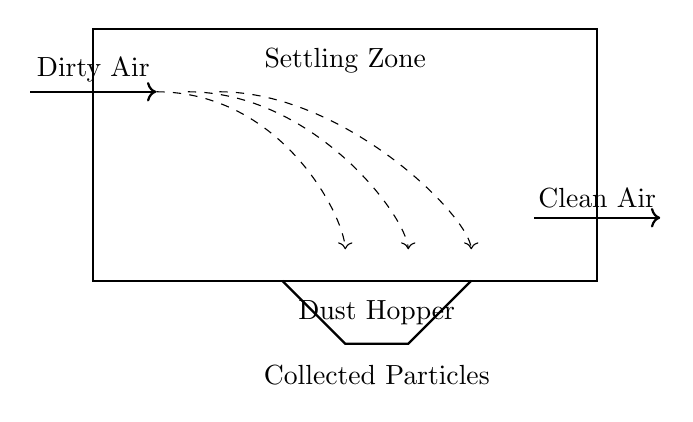
\begin{tikzpicture}[scale=0.8]
        % Chamber box
        \draw[thick] (0,0) rectangle (8,4);
        
        % Inlet
        \draw[thick, ->] (-1, 3) -- (1, 3) node[midway, above] {Dirty Air};
        
        % Outlet
        \draw[thick, ->] (7, 1) -- (9, 1) node[midway, above] {Clean Air};
        
        % Particles path
        \draw[dashed, ->] (1, 3) .. controls (3, 3) and (4, 1) .. (4, 0.5);
        \draw[dashed, ->] (1.5, 3) .. controls (3.5, 3) and (5, 1) .. (5, 0.5);
        \draw[dashed, ->] (2, 3) .. controls (4, 3) and (6, 1) .. (6, 0.5);
        
        % Hopper
        \draw[thick] (3, 0) -- (4, -1) -- (5, -1) -- (6, 0);
        \node at (4.5, -0.5) {Dust Hopper};
        \node at (4.5, -1.5) {Collected Particles};
        
        % Labels
        \node at (4, 3.5) {Settling Zone};
    \end{tikzpicture}
    \end{center}

    \begin{answertable}{Working Principle}
    \begin{tabulary}{\linewidth}{L L}
        \toprule
        \textbf{Parameter} & \textbf{Description} \\
        \midrule
        \textbf{Mechanism} & Gravitational settling of particles \\
        \textbf{Efficiency} & 50-70\% for particles $>$50 $\mu$m \\
        \textbf{Velocity} & Low gas velocity allows settling \\
        \bottomrule
    \end{tabulary}
    \end{answertable}

    \begin{itemize}
        \item \textbf{Applications}: Cement, mining, metallurgy industries
        \item \textbf{Advantages}: Simple design, low maintenance cost
        \item \textbf{Limitations}: Ineffective for fine particles
    \end{itemize}

    \begin{mnemonicbox}Gravity Settles Heavy Particles\end{mnemonicbox}
\end{solutionbox}

\questionmarks{2}{c}{7}
\textbf{Describe solid waste management.}

\begin{solutionbox}
    \textbf{Solid Waste Management Hierarchy:}
    \begin{center}
    \begin{tikzpicture}[node distance=1.5cm, auto]
        \node (reduce) [gtu block] {Reduce};
        \node (reuse) [gtu block, right=of reduce] {Reuse};
        \node (recycle) [gtu block, right=of reuse] {Recycle};
        \node (recovery) [gtu block, right=of recycle] {Recovery};
        \node (disposal) [gtu block, right=of recovery] {Disposal};

        \draw [gtu arrow] (reduce) -- (reuse);
        \draw [gtu arrow] (reuse) -- (recycle);
        \draw [gtu arrow] (recycle) -- (recovery);
        \draw [gtu arrow] (recovery) -- (disposal);
    \end{tikzpicture}
    \end{center}

    \begin{answertable}{Solid Waste Management Methods}
    \begin{tabulary}{\linewidth}{L L L}
        \toprule
        \textbf{Method} & \textbf{Description} & \textbf{Advantages} \\
        \midrule
        \textbf{Landfill} & Controlled burial & Simple, cost-effective \\
        \textbf{Incineration} & High-temperature burning & Volume reduction \\
        \textbf{Composting} & Biological decomposition & Nutrient-rich fertilizer \\
        \textbf{Recycling} & Material recovery & Resource conservation \\
        \bottomrule
    \end{tabulary}
    \end{answertable}

    \textbf{Components:}
    \begin{itemize}
        \item \textbf{Collection}: Door-to-door pickup systems
        \item \textbf{Transportation}: Efficient vehicle routing
        \item \textbf{Treatment}: Sorting, processing, disposal
        \item \textbf{Monitoring}: Regular quality checks
    \end{itemize}

    \begin{mnemonicbox}Collect, Transport, Treat, Monitor\end{mnemonicbox}
\end{solutionbox}

\questionmarks{2}{a}{3}
\textbf{Write effect on noise pollution.}

\begin{solutionbox}
    \begin{answertable}{Effects of Noise Pollution}
    \begin{tabulary}{\linewidth}{L L}
        \toprule
        \textbf{Type} & \textbf{Effects} \\
        \midrule
        \textbf{Health Effects} & Hearing loss, stress, hypertension \\
        \textbf{Psychological} & Irritation, sleep disorders, anxiety \\
        \textbf{Environmental} & Wildlife disruption, ecosystem damage \\
        \bottomrule
    \end{tabulary}
    \end{answertable}

    \begin{itemize}
        \item \textbf{Sources}: Traffic, industries, construction, aircraft
        \item \textbf{Measurement}: Decibel (dB) scale
        \item \textbf{Control}: Sound barriers, noise regulations
    \end{itemize}

    \begin{mnemonicbox}Noise Harms Health and Habitat\end{mnemonicbox}
\end{solutionbox}

\questionmarks{2}{b}{4}
\textbf{What is water pollution? Write list of main water pollutant?}

\begin{solutionbox}
    \textbf{Water Pollution Definition:}
    Contamination of water bodies by harmful substances making it unsuitable for use.

    \begin{answertable}{Major Water Pollutants}
    \begin{tabulary}{\linewidth}{L L}
        \toprule
        \textbf{Category} & \textbf{Examples} \\
        \midrule
        \textbf{Chemical} & Heavy metals, pesticides, fertilizers \\
        \textbf{Biological} & Bacteria, viruses, parasites \\
        \textbf{Physical} & Suspended solids, thermal pollution \\
        \textbf{Radioactive} & Nuclear waste materials \\
        \bottomrule
    \end{tabulary}
    \end{answertable}

    \begin{itemize}
        \item \textbf{Sources}: Industrial discharge, domestic sewage, agricultural runoff
        \item \textbf{Effects}: Disease transmission, ecosystem disruption
        \item \textbf{Control}: Treatment plants, pollution prevention
    \end{itemize}

    \begin{mnemonicbox}Chemical, Biological, Physical, Radioactive\end{mnemonicbox}
\end{solutionbox}

\questionmarks{2}{c}{7}
\textbf{What is E-waste? Write impact of E-waste on environment and human health. How to recycle E-waste?}

\begin{solutionbox}
    \textbf{E-waste Definition:}
    Electronic waste includes discarded electrical and electronic devices.

    \textbf{Environmental Impact:}
    \begin{center}
    \begin{tikzpicture}[node distance=1.5cm, auto]
        \node (ewaste) [gtu block] {E-waste};
        \node (soil) [gtu block, below left=of ewaste] {Soil Contamination};
        \node (water) [gtu block, below right=of ewaste] {Water Pollution};
        \node (air) [gtu block, above right=of ewaste] {Air Pollution};
        \node (resource) [gtu block, above left=of ewaste] {Resource Depletion};

        \draw [gtu arrow] (ewaste) -- (soil);
        \draw [gtu arrow] (ewaste) -- (water);
        \draw [gtu arrow] (ewaste) -- (air);
        \draw [gtu arrow] (ewaste) -- (resource);
    \end{tikzpicture}
    \end{center}

    \begin{answertable}{Health Impact of E-waste}
    \begin{tabulary}{\linewidth}{L L}
        \toprule
        \textbf{Toxic Material} & \textbf{Health Effects} \\
        \midrule
        \textbf{Lead} & Nervous system damage \\
        \textbf{Mercury} & Brain and kidney damage \\
        \textbf{Cadmium} & Cancer, lung damage \\
        \bottomrule
    \end{tabulary}
    \end{answertable}

    \textbf{E-waste Recycling Process:}
    \begin{itemize}
        \item \textbf{Collection}: Designated collection centers
        \item \textbf{Dismantling}: Manual separation of components
        \item \textbf{Recovery}: Extraction of valuable materials
        \item \textbf{Disposal}: Safe handling of toxic substances
    \end{itemize}

    \begin{mnemonicbox}Collect, Dismantle, Recover, Dispose Safely\end{mnemonicbox}
\end{solutionbox}

\questionmarks{3}{a}{3}
\textbf{What is BOD? Give a importance of BOD.}

\begin{solutionbox}
    \begin{answertable}{BOD Parameters}
    \begin{tabulary}{\linewidth}{L L}
        \toprule
        \textbf{Parameter} & \textbf{Description} \\
        \midrule
        \textbf{Definition} & Oxygen required by microorganisms to decompose organic matter \\
        \textbf{Unit} & mg/L or ppm \\
        \textbf{Test Period} & 5 days at 20$^{\circ}$C \\
        \bottomrule
    \end{tabulary}
    \end{answertable}

    \textbf{Importance:}
    \begin{itemize}
        \item \textbf{Water Quality}: Indicates organic pollution level
        \item \textbf{Treatment Efficiency}: Monitors treatment plant performance
        \item \textbf{Environmental Health}: Assesses aquatic ecosystem condition
    \end{itemize}

    \begin{mnemonicbox}Bacteria Oxygen Demand measures pollution\end{mnemonicbox}
\end{solutionbox}

\questionmarks{3}{b}{4}
\textbf{Give a comparison of conventional and Non conventional energy sources.}

\begin{solutionbox}
    \begin{answertable}{Energy Sources Comparison}
    \begin{tabulary}{\linewidth}{L L L}
        \toprule
        \textbf{Parameter} & \textbf{Conventional} & \textbf{Non-Conventional} \\
        \midrule
        \textbf{Examples} & Coal, oil, natural gas & Solar, wind, biomass \\
        \textbf{Availability} & Limited reserves & Unlimited/renewable \\
        \textbf{Environment} & High pollution & Environment friendly \\
        \textbf{Cost} & Initially cheap & High initial cost \\
        \textbf{Sustainability} & Non-sustainable & Sustainable \\
        \bottomrule
    \end{tabulary}
    \end{answertable}

    \begin{itemize}
        \item \textbf{Conventional}: Depleting rapidly, cause greenhouse gases
        \item \textbf{Non-conventional}: Clean, abundant, future energy solution
        \item \textbf{Transition}: Global shift towards renewable energy
    \end{itemize}

    \begin{mnemonicbox}Conventional Pollutes, Renewable Sustains\end{mnemonicbox}
\end{solutionbox}

\questionmarks{3}{c}{7}
\textbf{Give classification of wind turbines and explain horizontal axis wind turbine.}

\begin{solutionbox}
    \textbf{Wind Turbine Classification:}
    \begin{center}
    \begin{tikzpicture}[node distance=1.5cm, auto, align=center]
        \node (root) [gtu block] {Wind Turbines};
        \node (hawt) [gtu block, below left=of root, xshift=-1cm] {Horizontal Axis\\(HAWT)};
        \node (vawt) [gtu block, below right=of root, xshift=1cm] {Vertical Axis\\(VAWT)};
        
        \node (upwind) [gtu state, below left=of hawt] {Upwind};
        \node (downwind) [gtu state, below right=of hawt] {Downwind};
        
        \node (darrieus) [gtu state, below left=of vawt] {Darrieus};
        \node (savonius) [gtu state, below right=of vawt] {Savonius};

        \draw [gtu arrow] (root) -- (hawt);
        \draw [gtu arrow] (root) -- (vawt);
        \draw [gtu arrow] (hawt) -- (upwind);
        \draw [gtu arrow] (hawt) -- (downwind);
        \draw [gtu arrow] (vawt) -- (darrieus);
        \draw [gtu arrow] (vawt) -- (savonius);
    \end{tikzpicture}
    \end{center}

    \textbf{Horizontal Axis Wind Turbine (HAWT):}

    \begin{answertable}{HAWT Components}
    \begin{tabulary}{\linewidth}{L L}
        \toprule
        \textbf{Component} & \textbf{Function} \\
        \midrule
        \textbf{Rotor Blades} & Convert wind energy to rotational motion \\
        \textbf{Nacelle} & Houses generator and gearbox \\
        \textbf{Tower} & Supports turbine at optimal height \\
        \textbf{Foundation} & Provides structural stability \\
        \bottomrule
    \end{tabulary}
    \end{answertable}

    \textbf{Working Principle:}
    \begin{itemize}
        \item \textbf{Wind Direction}: Parallel to rotor axis
        \item \textbf{Blade Design}: Aerodynamic lift principle
        \item \textbf{Power Generation}: Variable speed operation
        \item \textbf{Efficiency}: 35-45\% energy conversion
    \end{itemize}

    \textbf{Advantages:}
    \begin{itemize}
        \item \textbf{High Efficiency}: Better power coefficient
        \item \textbf{Mature Technology}: Well-established design
        \item \textbf{Cost Effective}: Lower maintenance costs
    \end{itemize}

    \begin{mnemonicbox}Horizontal High Efficiency\end{mnemonicbox}
\end{solutionbox}


\questionmarks{3}{a}{3}
\textbf{Explain need for renewable energy.}

\begin{solutionbox}
    \begin{answertable}{Need for Renewable Energy}
    \begin{tabulary}{\linewidth}{L L}
        \toprule
        \textbf{Reason} & \textbf{Description} \\
        \midrule
        \textbf{Energy Security} & Reduce import dependence \\
        \textbf{Environmental Protection} & Zero carbon emissions \\
        \textbf{Economic Benefits} & Job creation, cost reduction \\
        \bottomrule
    \end{tabulary}
    \end{answertable}

    \begin{itemize}
        \item \textbf{Fossil Fuel Depletion}: Limited reserves, increasing prices
        \item \textbf{Climate Change}: Urgent need to reduce greenhouse gases
        \item \textbf{Sustainable Development}: Meet present needs without compromising future
    \end{itemize}

    \begin{mnemonicbox}Security, Environment, Economy need Renewables\end{mnemonicbox}
\end{solutionbox}

\questionmarks{3}{b}{4}
\textbf{Write a short note on Geo thermal energy.}

\begin{solutionbox}
    \textbf{Geothermal Energy:}
    Heat energy stored beneath Earth's surface used for power generation.

    \begin{answertable}{Geothermal Energy Types}
    \begin{tabulary}{\linewidth}{L L L}
        \toprule
        \textbf{Type} & \textbf{Temperature} & \textbf{Application} \\
        \midrule
        \textbf{High Temperature} & $>$150$^{\circ}$C & Power generation \\
        \textbf{Medium Temperature} & 90-150$^{\circ}$C & Direct heating \\
        \textbf{Low Temperature} & $<$90$^{\circ}$C & Heat pumps \\
        \bottomrule
    \end{tabulary}
    \end{answertable}

    \begin{itemize}
        \item \textbf{Sources}: Hot springs, geysers, underground reservoirs
        \item \textbf{Advantages}: Continuous availability, low emissions
        \item \textbf{Applications}: Electricity generation, space heating, industrial processes
    \end{itemize}

    \begin{mnemonicbox}Earth's Heat Powers Homes\end{mnemonicbox}
\end{solutionbox}

\questionmarks{3}{c}{7}
\textbf{Explain the principal and working of solar photovoltaic cell. Give its uses.}

\begin{solutionbox}
    \textbf{Solar Photovoltaic Cell Principle:}
    Converts sunlight directly into electricity using photovoltaic effect.

    \textbf{Working Process:}
    \begin{center}
    \begin{tikzpicture}[node distance=1.5cm, auto]
        \node (sun) [gtu block] {Sunlight};
        \node (silicon) [gtu block, right=of sun] {Silicon Cell};
        \node (electron) [gtu block, right=of silicon] {Electron Movement};
        \node (current) [gtu block, below=of electron] {Electric Current};
        \node (dc) [gtu block, left=of current] {DC Power};
        \node (inverter) [gtu block, left=of dc] {Inverter};
        \node (ac) [gtu block, below=of inverter] {AC Power};

        \draw [gtu arrow] (sun) -- (silicon);
        \draw [gtu arrow] (silicon) -- (electron);
        \draw [gtu arrow] (electron) -- (current);
        \draw [gtu arrow] (current) -- (dc);
        \draw [gtu arrow] (dc) -- (inverter);
        \draw [gtu arrow] (inverter) -- (ac);
    \end{tikzpicture}
    \end{center}

    \begin{answertable}{Solar Cell Structure}
    \begin{tabulary}{\linewidth}{L L L}
        \toprule
        \textbf{Layer} & \textbf{Material} & \textbf{Function} \\
        \midrule
        \textbf{Top Layer} & N-type silicon & Excess electrons \\
        \textbf{Bottom Layer} & P-type silicon & Electron holes \\
        \textbf{Junction} & P-N junction & Electric field creation \\
        \bottomrule
    \end{tabulary}
    \end{answertable}

    \textbf{Working Steps:}
    \begin{itemize}
        \item \textbf{Photon Absorption}: Light energy absorbed by silicon
        \item \textbf{Electron Excitation}: Electrons gain energy and move
        \item \textbf{Current Generation}: Electron flow creates electricity
        \item \textbf{External Circuit}: Current flows through load
    \end{itemize}

    \textbf{Applications:}
    \begin{itemize}
        \item \textbf{Residential}: Rooftop solar systems
        \item \textbf{Commercial}: Solar farms, street lighting
        \item \textbf{Industrial}: Remote power supply, satellites
        \item \textbf{Transportation}: Solar vehicles, charging stations
    \end{itemize}

    \textbf{Advantages:}
    \begin{itemize}
        \item \textbf{Clean Energy}: No emissions during operation
        \item \textbf{Low Maintenance}: Minimal moving parts
        \item \textbf{Modular}: Scalable installation
    \end{itemize}

    \begin{mnemonicbox}Sun Strikes Silicon, Sparks Current\end{mnemonicbox}
\end{solutionbox}

\questionmarks{4}{a}{3}
\textbf{Explain Green house effect.}

\begin{solutionbox}
    \textbf{Greenhouse Effect:}
    Natural process where certain gases trap heat in Earth's atmosphere.

    \begin{answertable}{Greenhouse Effect Mechanism}
    \begin{tabulary}{\linewidth}{L L}
        \toprule
        \textbf{Step} & \textbf{Process} \\
        \midrule
        \textbf{Solar Radiation} & Sun's energy reaches Earth \\
        \textbf{Surface Absorption} & Earth absorbs and heats up \\
        \textbf{Re-radiation} & Earth emits infrared radiation \\
        \textbf{Gas Trapping} & Greenhouse gases trap heat \\
        \bottomrule
    \end{tabulary}
    \end{answertable}

    \begin{itemize}
        \item \textbf{Natural Effect}: Maintains Earth's temperature for life
        \item \textbf{Enhanced Effect}: Human activities increase greenhouse gases
        \item \textbf{Result}: Global warming and climate change
    \end{itemize}

    \begin{mnemonicbox}Gases Trap Heat, Earth Heats\end{mnemonicbox}
\end{solutionbox}

\questionmarks{4}{b}{4}
\textbf{Write international protocol to prevent climate change management.}

\begin{solutionbox}
    \begin{answertable}{International Climate Protocols}
    \begin{tabulary}{\linewidth}{L L L}
        \toprule
        \textbf{Protocol} & \textbf{Year} & \textbf{Objective} \\
        \midrule
        \textbf{Kyoto Protocol} & 1997 & Reduce greenhouse gas emissions \\
        \textbf{Paris Agreement} & 2015 & Limit global warming to 1.5$^{\circ}$C \\
        \textbf{Montreal Protocol} & 1987 & Protect ozone layer \\
        \bottomrule
    \end{tabulary}
    \end{answertable}

    \textbf{Key Features:}
    \begin{itemize}
        \item \textbf{Emission Targets}: Binding commitments for developed countries
        \item \textbf{Clean Development}: Technology transfer to developing nations
        \item \textbf{Carbon Trading}: Market-based emission reduction mechanisms
        \item \textbf{Monitoring}: Regular reporting and verification systems
    \end{itemize}

    \begin{mnemonicbox}Kyoto, Paris, Montreal Protect Climate\end{mnemonicbox}
\end{solutionbox}

\questionmarks{4}{c}{7}
\textbf{Explain biogas plant with neat sketch.}

\begin{solutionbox}
    \textbf{Biogas Plant:}
    \begin{center}
    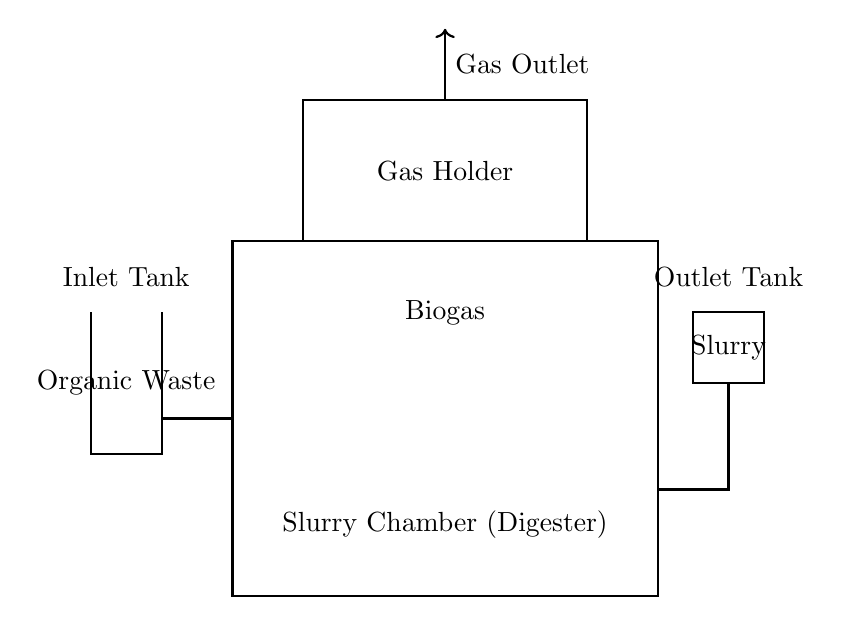
\begin{tikzpicture}[scale=0.9]
        % Inlet tank
        \draw[thick] (0,2) -- (0,0) -- (1,0) -- (1,2);
        \node at (0.5, 2.5) {Inlet Tank};
        \node at (0.5, 1) {Organic Waste};
        
        % Pipe to digester
        \draw[thick] (1,0.5) -- (2,0.5) -- (2,-2);
        
        % Digester
        \draw[thick] (2,-2) rectangle (8,3);
        \node at (5, -1) {Slurry Chamber (Digester)};
        
        % Gas holder
        \draw[thick] (3,3) -- (3,5) -- (7,5) -- (7,3);
        \node at (5, 4) {Gas Holder};
        
        % Gas outlet
        \draw[thick, ->] (5, 5) -- (5, 6) node[midway, right] {Gas Outlet};
        
        % Outlet pipe
        \draw[thick] (8,-0.5) -- (9,-0.5) -- (9,1);
        \draw[thick] (8.5, 1) rectangle (9.5, 2);
        \node at (9, 2.5) {Outlet Tank};
        \node at (9, 1.5) {Slurry};

        % Labels
        \node at (5, 2) {Biogas};
    \end{tikzpicture}
    \end{center}

    \begin{answertable}{Biogas Plant Components}
    \begin{tabulary}{\linewidth}{L L}
        \toprule
        \textbf{Component} & \textbf{Function} \\
        \midrule
        \textbf{Inlet Tank} & Receives organic waste \\
        \textbf{Digester} & Anaerobic decomposition occurs \\
        \textbf{Gas Holder} & Stores produced biogas \\
        \textbf{Outlet} & Removes spent slurry \\
        \bottomrule
    \end{tabulary}
    \end{answertable}

    \textbf{Working Process:}
    \begin{itemize}
        \item \textbf{Loading}: Organic waste mixed with water
        \item \textbf{Digestion}: Bacteria decompose waste anaerobically
        \item \textbf{Gas Production}: Methane and CO$_2$ generated
        \item \textbf{Collection}: Gas stored in holder for use
    \end{itemize}

    \textbf{Raw Materials:}
    \begin{itemize}
        \item \textbf{Animal Waste}: Cow dung, poultry droppings
        \item \textbf{Plant Waste}: Agricultural residues, kitchen waste
        \item \textbf{Water}: Maintains proper consistency
    \end{itemize}

    \textbf{Products:}
    \begin{itemize}
        \item \textbf{Biogas}: 50-70\% methane for cooking/heating
        \item \textbf{Slurry}: Excellent organic fertilizer
    \end{itemize}

    \textbf{Advantages:}
    \begin{itemize}
        \item \textbf{Renewable}: Continuous gas production
        \item \textbf{Waste Management}: Converts waste to energy
        \item \textbf{Rural Development}: Suitable for villages
    \end{itemize}

    \begin{mnemonicbox}Waste In, Gas Out, Fertilizer Bonus\end{mnemonicbox}
\end{solutionbox}

\questionmarks{4}{a}{3}
\textbf{Write short note on green house gases.}

\begin{solutionbox}
    \begin{answertable}{Greenhouse Gases Details}
    \begin{tabulary}{\linewidth}{L L L}
        \toprule
        \textbf{Gas} & \textbf{Source} & \textbf{Contribution} \\
        \midrule
        \textbf{Carbon Dioxide} & Fossil fuels, deforestation & 76\% \\
        \textbf{Methane} & Agriculture, landfills & 16\% \\
        \textbf{Nitrous Oxide} & Fertilizers, combustion & 6\% \\
        \textbf{Fluorinated Gases} & Industrial processes & 2\% \\
        \bottomrule
    \end{tabulary}
    \end{answertable}

    \begin{itemize}
        \item \textbf{Properties}: Absorb and emit infrared radiation
        \item \textbf{Impact}: Trap heat causing global warming
        \item \textbf{Control}: Reduce emissions, use alternatives
    \end{itemize}

    \begin{mnemonicbox}CO2, CH4, N2O, F-gases Heat Earth\end{mnemonicbox}
\end{solutionbox}

\questionmarks{4}{b}{4}
\textbf{Explain ozone layer depletion.}

\begin{solutionbox}
    \textbf{Ozone Layer Depletion:}
    Reduction of ozone concentration in stratosphere due to human activities.

    \begin{answertable}{Causes of Ozone Depletion}
    \begin{tabulary}{\linewidth}{L L L}
        \toprule
        \textbf{Substance} & \textbf{Source} & \textbf{Effect} \\
        \midrule
        \textbf{CFCs} & Refrigerants, aerosols & Break down ozone molecules \\
        \textbf{Halons} & Fire extinguishers & Catalytic ozone destruction \\
        \textbf{Methyl Bromide} & Pesticides & Ozone layer thinning \\
        \bottomrule
    \end{tabulary}
    \end{answertable}

    \textbf{Process:}
    \begin{itemize}
        \item \textbf{UV Breakdown}: UV radiation breaks CFC molecules
        \item \textbf{Chlorine Release}: Free chlorine atoms released
        \item \textbf{Ozone Destruction}: Chlorine destroys ozone molecules
        \item \textbf{Chain Reaction}: One CFC molecule destroys many ozone molecules
    \end{itemize}

    \textbf{Effects}: Increased UV radiation, skin cancer, crop damage

    \begin{mnemonicbox}CFCs Climb, Chlorine Chops Ozone\end{mnemonicbox}
\end{solutionbox}

\questionmarks{4}{c}{7}
\textbf{Explain the term "climate changes and state its causes and effects"}

\begin{solutionbox}
    \textbf{Climate Change Definition:}
    Long-term shifts in global weather patterns and temperatures.

    \textbf{Causes:}
    \begin{center}
    \begin{tikzpicture}[node distance=1.5cm, auto, align=center]
        \node (clim) [gtu block] {Climate Change\\Causes};
        \node (nat) [gtu block, below left=of clim] {Natural};
        \node (human) [gtu block, below right=of clim] {Human Activities};
        
        \node (solar) [gtu state, below=of nat, xshift=-1cm] {Solar Variations};
        \node (volc) [gtu state, below=of nat, xshift=1cm] {Volcanic\\Eruptions};
        
        \node (ghg) [gtu state, below=of human, xshift=-1cm] {GHG Emissions};
        \node (defor) [gtu state, below=of human, xshift=1cm] {Deforestation};
        \node (ind) [gtu state, below=of human, yshift=-1.5cm] {Industrial\\Activities};

        \draw [gtu arrow] (clim) -- (nat);
        \draw [gtu arrow] (clim) -- (human);
        \draw [gtu arrow] (nat) -- (solar);
        \draw [gtu arrow] (nat) -- (volc);
        \draw [gtu arrow] (human) -- (ghg);
        \draw [gtu arrow] (human) -- (defor);
        \draw [gtu arrow] (human) -- (ind);
    \end{tikzpicture}
    \end{center}

    \begin{answertable}{Human Causes of Climate Change}
    \begin{tabulary}{\linewidth}{L L}
        \toprule
        \textbf{Activity} & \textbf{Contribution} \\
        \midrule
        \textbf{Fossil Fuel Burning} & 65\% of CO$_2$ emissions \\
        \textbf{Deforestation} & 15\% of emissions \\
        \textbf{Industrial Processes} & 20\% of emissions \\
        \bottomrule
    \end{tabulary}
    \end{answertable}

    \textbf{Effects:}
    
    \textbf{Environmental Effects:}
    \begin{itemize}
        \item \textbf{Temperature Rise}: Global average temperature increase
        \item \textbf{Sea Level Rise}: Thermal expansion and ice melting
        \item \textbf{Weather Extremes}: More frequent droughts, floods
    \end{itemize}

    \textbf{Biological Effects:}
    \begin{itemize}
        \item \textbf{Species Migration}: Animals moving to cooler regions
        \item \textbf{Ecosystem Disruption}: Food chain alterations
        \item \textbf{Biodiversity Loss}: Species extinction rates increase
    \end{itemize}

    \textbf{Human Effects:}
    \begin{itemize}
        \item \textbf{Agriculture}: Crop yield changes, food security issues
        \item \textbf{Health}: Heat stress, disease vector changes
        \item \textbf{Economy}: Infrastructure damage, adaptation costs
    \end{itemize}

    \textbf{Mitigation Strategies:}
    \begin{itemize}
        \item \textbf{Renewable Energy}: Transition from fossil fuels
        \item \textbf{Energy Efficiency}: Reduce consumption
        \item \textbf{Carbon Sequestration}: Forest conservation, tree planting
        \item \textbf{International Cooperation}: Global agreements and policies
    \end{itemize}

    \begin{mnemonicbox}Human Actions Heat Earth, Everyone Affected\end{mnemonicbox}
\end{solutionbox}

\questionmarks{5}{a}{3}
\textbf{Explain "Khet Talavadi".}

\begin{solutionbox}
    \textbf{Khet Talavadi (Farm Pond):}
    Small water harvesting structure in agricultural fields for irrigation.

    \begin{answertable}{Farm Pond Features}
    \begin{tabulary}{\linewidth}{L L}
        \toprule
        \textbf{Parameter} & \textbf{Description} \\
        \midrule
        \textbf{Size} & 20m x 20m x 3m depth \\
        \textbf{Capacity} & 1200 cubic meters \\
        \textbf{Cost} & Subsidized by government \\
        \bottomrule
    \end{tabulary}
    \end{answertable}

    \begin{itemize}
        \item \textbf{Purpose}: Rainwater collection, irrigation during dry periods
        \item \textbf{Benefits}: Increased crop yield, groundwater recharge
        \item \textbf{Construction}: Lined with plastic sheets or cement
    \end{itemize}

    \begin{mnemonicbox}Farm Pond Stores Rain for Crops\end{mnemonicbox}
\end{solutionbox}

\questionmarks{5}{b}{4}
\textbf{Give goal and advantage of green building.}

\begin{solutionbox}
    \begin{answertable}{Green Building Goals}
    \begin{tabulary}{\linewidth}{L L}
        \toprule
        \textbf{Goal} & \textbf{Description} \\
        \midrule
        \textbf{Energy Efficiency} & Reduce energy consumption \\
        \textbf{Water Conservation} & Minimize water usage \\
        \textbf{Material Efficiency} & Use sustainable materials \\
        \textbf{Indoor Environment} & Improve air quality \\
        \bottomrule
    \end{tabulary}
    \end{answertable}

    \textbf{Advantages:}
    \begin{itemize}
        \item \textbf{Environmental}: Reduced carbon footprint, waste minimization
        \item \textbf{Economic}: Lower operating costs, increased property value
        \item \textbf{Health}: Better indoor air quality, natural lighting
        \item \textbf{Social}: Enhanced occupant comfort, productivity
    \end{itemize}

    \textbf{Green Building Features:}
    \begin{itemize}
        \item \textbf{Solar Panels}: Renewable energy generation
        \item \textbf{Rainwater Harvesting}: Water conservation
        \item \textbf{Green Roofs}: Insulation and air purification
    \end{itemize}

    \begin{mnemonicbox}Green Goals: Energy, Water, Materials, Environment\end{mnemonicbox}
\end{solutionbox}

\questionmarks{5}{c}{7}
\textbf{Explain various methods of rain water harvesting.}

\begin{solutionbox}
    \textbf{Rainwater Harvesting Methods:}

    \textbf{Surface Methods:}
    \begin{center}
    \begin{tikzpicture}[node distance=1.5cm, auto, align=center]
        \node (root) [gtu block] {Rainwater Harvesting};
        \node (surf) [gtu block, below left=of root, xshift=-1cm] {Surface Methods};
        \node (ground) [gtu block, below right=of root, xshift=1cm] {Groundwater Methods};
        
        \node (pond) [gtu state, below left=of surf] {Ponds \& Tanks};
        \node (dam) [gtu state, below right=of surf] {Check Dams};
        
        \node (pit) [gtu state, below left=of ground] {Percolation Pits};
        \node (well) [gtu state, below right=of ground] {Recharge Wells};

        \draw [gtu arrow] (root) -- (surf);
        \draw [gtu arrow] (root) -- (ground);
        \draw [gtu arrow] (surf) -- (pond);
        \draw [gtu arrow] (surf) -- (dam);
        \draw [gtu arrow] (ground) -- (pit);
        \draw [gtu arrow] (ground) -- (well);
    \end{tikzpicture}
    \end{center}

    \begin{answertable}{Detailed Rainwater Harvesting Methods}
    \begin{tabulary}{\linewidth}{L L L}
        \toprule
        \textbf{Method} & \textbf{Description} & \textbf{Application} \\
        \midrule
        \textbf{Rooftop Harvesting} & Collect water from building roofs & Urban areas \\
        \textbf{Surface Runoff} & Capture water from ground surface & Rural areas \\
        \textbf{Check Dams} & Small barriers across streams & Hilly regions \\
        \textbf{Percolation Tanks} & Allow water to seep underground & Groundwater recharge \\
        \bottomrule
    \end{tabulary}
    \end{answertable}

    \textbf{System Components:}
    \begin{itemize}
        \item \textbf{Catchment Area}: Surface collecting rainwater
        \item \textbf{Conveyance System}: Gutters, pipes for transport
        \item \textbf{Storage System}: Tanks, ponds for holding water
        \item \textbf{Filter System}: Remove debris and contaminants
    \end{itemize}

    \textbf{Rooftop Harvesting Process:}
    \begin{itemize}
        \item \textbf{Collection}: Rain falls on roof surface
        \item \textbf{Conveyance}: Water flows through gutters and downspouts
        \item \textbf{First Flush}: Initial dirty water diverted
        \item \textbf{Storage}: Clean water stored in tanks
        \item \textbf{Distribution}: Water used for various purposes
    \end{itemize}

    \textbf{Benefits:}
    \begin{itemize}
        \item \textbf{Water Security}: Reduce dependence on external supply
        \item \textbf{Flood Control}: Reduce surface runoff and flooding
        \item \textbf{Groundwater Recharge}: Replenish underground aquifers
        \item \textbf{Cost Savings}: Reduce water bills
    \end{itemize}

    \textbf{Design Considerations:}
    \begin{itemize}
        \item \textbf{Rainfall Data}: Annual precipitation patterns
        \item \textbf{Catchment Area}: Available roof/ground area
        \item \textbf{Storage Capacity}: Based on demand and supply
        \item \textbf{Water Quality}: Treatment requirements
    \end{itemize}

    \begin{mnemonicbox}Catch, Convey, Store, Filter, Use\end{mnemonicbox}
\end{solutionbox}

\questionmarks{5}{a}{3}
\textbf{What is Life cycle analysis (LCA)?}

\begin{solutionbox}
    \textbf{Life Cycle Analysis (LCA):}
    Systematic evaluation of environmental impacts of a product throughout its entire life cycle.

    \textbf{LCA Stages:}
    \begin{answertable}{LCA Stages}
    \begin{tabulary}{\linewidth}{L L}
        \toprule
        \textbf{Stage} & \textbf{Description} \\
        \midrule
        \textbf{Raw Material} & Resource extraction \\
        \textbf{Manufacturing} & Production processes \\
        \textbf{Use Phase} & Product utilization \\
        \textbf{End of Life} & Disposal or recycling \\
        \bottomrule
    \end{tabulary}
    \end{answertable}

    \begin{itemize}
        \item \textbf{Purpose}: Identify environmental hotspots, compare alternatives
        \item \textbf{Applications}: Product design, policy decisions, consumer choices
    \end{itemize}

    \begin{mnemonicbox}Life Cycle: Raw, Make, Use, Dispose\end{mnemonicbox}
\end{solutionbox}

\questionmarks{5}{b}{4}
\textbf{Give main features of the biological diversity Act, 2002}

\begin{solutionbox}
    \textbf{Biological Diversity Act, 2002:}

    \begin{answertable}{Main Features}
    \begin{tabulary}{\linewidth}{L L}
        \toprule
        \textbf{Feature} & \textbf{Description} \\
        \midrule
        \textbf{Three-tier Structure} & National, State, Local Biodiversity Boards \\
        \textbf{Prior Approval} & Required for bio-resource access \\
        \textbf{Benefit Sharing} & Equitable sharing with local communities \\
        \textbf{Bio-piracy Prevention} & Protect traditional knowledge \\
        \bottomrule
    \end{tabulary}
    \end{answertable}

    \textbf{Key Provisions:}
    \begin{itemize}
        \item \textbf{Access Regulation}: Control over biological resources
        \item \textbf{Sustainable Use}: Conservation through utilization
        \item \textbf{Community Rights}: Recognize local community contributions
        \item \textbf{Penalties}: Strict punishment for violations
    \end{itemize}

    \textbf{Objectives}: Conservation, sustainable use, equitable benefit sharing

    \begin{mnemonicbox}Biodiversity Act: Access, Benefit, Conserve, Protect\end{mnemonicbox}
\end{solutionbox}

\questionmarks{5}{c}{7}
\textbf{Explain 5R.}

\begin{solutionbox}
    \textbf{5R Concept:}
    Waste management hierarchy for environmental sustainability.

    \textbf{The 5Rs:}
    \begin{center}
    \begin{tikzpicture}[node distance=1.5cm, auto]
        \node (r5) [gtu block] {5R Hierarchy};
        \node (refuse) [gtu block, below=of r5] {1. Refuse};
        \node (reduce) [gtu block, below=of refuse] {2. Reduce};
        \node (reuse) [gtu block, below=of reduce] {3. Reuse};
        \node (repurpose) [gtu block, below=of reuse] {4. Repurpose};
        \node (recycle) [gtu block, below=of repurpose] {5. Recycle};

        \draw [gtu arrow] (r5) -- (refuse);
        \draw [gtu arrow] (refuse) -- (reduce);
        \draw [gtu arrow] (reduce) -- (reuse);
        \draw [gtu arrow] (reuse) -- (repurpose);
        \draw [gtu arrow] (repurpose) -- (recycle);
    \end{tikzpicture}
    \end{center}

    \begin{answertable}{Detailed Explanation of 5Rs}
    \begin{tabulary}{\linewidth}{L L L L}
        \toprule
        \textbf{R} & \textbf{Definition} & \textbf{Examples} & \textbf{Benefits} \\
        \midrule
        \textbf{Refuse} & Avoid unnecessary items & Plastic bags, disposables & Prevent waste generation \\
        \textbf{Reduce} & Minimize consumption & Energy, water, materials & Lower resource demand \\
        \textbf{Reuse} & Use items multiple times & Containers, clothing & Extend product life \\
        \textbf{Repurpose} & Find new uses for items & Tire planters, bottle crafts & Creative waste diversion \\
        \textbf{Recycle} & Process into new products & Paper, plastic, metals & Material recovery \\
        \bottomrule
    \end{tabulary}
    \end{answertable}

    \textbf{Implementation Strategies:}
    
    \textbf{Personal Level:}
    \begin{itemize}
        \item \textbf{Refuse}: Say no to single-use plastics
        \item \textbf{Reduce}: Buy only necessary items
        \item \textbf{Reuse}: Repurpose containers and materials
        \item \textbf{Repurpose}: Creative DIY projects
        \item \textbf{Recycle}: Proper sorting and disposal
    \end{itemize}

    \textbf{Community Level:}
    \begin{itemize}
        \item \textbf{Awareness Programs}: Education about 5R principles
        \item \textbf{Infrastructure}: Recycling facilities and collection systems
        \item \textbf{Policies}: Regulations promoting waste reduction
        \item \textbf{Incentives}: Rewards for sustainable practices
    \end{itemize}

    \textbf{Industrial Level:}
    \begin{itemize}
        \item \textbf{Design for Durability}: Long-lasting products
        \item \textbf{Material Selection}: Recyclable and biodegradable materials
        \item \textbf{Circular Economy}: Closed-loop production systems
        \item \textbf{Extended Producer Responsibility}: Manufacturer accountability
    \end{itemize}

    \textbf{Environmental Benefits:}
    \begin{itemize}
        \item \textbf{Resource Conservation}: Reduced raw material extraction
        \item \textbf{Energy Savings}: Lower production energy requirements
        \item \textbf{Pollution Reduction}: Decreased waste generation
        \item \textbf{Climate Protection}: Reduced greenhouse gas emissions
    \end{itemize}

    \textbf{Economic Benefits:}
    \begin{itemize}
        \item \textbf{Cost Savings}: Lower disposal and material costs
        \item \textbf{Job Creation}: Green jobs in recycling and reuse sectors
        \item \textbf{Innovation}: Development of sustainable technologies
        \item \textbf{Market Opportunities}: New business models
    \end{itemize}

    \textbf{Social Benefits:}
    \begin{itemize}
        \item \textbf{Community Engagement}: Collective environmental action
        \item \textbf{Health Improvement}: Cleaner environment
        \item \textbf{Education}: Environmental awareness and responsibility
        \item \textbf{Cultural Change}: Sustainable lifestyle adoption
    \end{itemize}

    \textbf{Challenges:}
    \begin{itemize}
        \item \textbf{Behavior Change}: Overcoming consumption habits
        \item \textbf{Infrastructure}: Adequate recycling facilities
        \item \textbf{Economic Barriers}: Initial investment requirements
        \item \textbf{Policy Support}: Government regulations and incentives
    \end{itemize}

    \textbf{Success Stories:}
    \begin{itemize}
        \item \textbf{Zero Waste Cities}: San Francisco, Kamikatsu
        \item \textbf{Corporate Initiatives}: Company 5R programs
        \item \textbf{School Programs}: Student environmental education
        \item \textbf{Community Projects}: Local waste reduction efforts
    \end{itemize}

    \begin{mnemonicbox}Really Reduce Reuse Repurpose Recycle\end{mnemonicbox}
\end{solutionbox}

\end{document}
